\documentclass[sigconf]{acmart}
\settopmatter{printacmref=false} % Removes citation information below abstract
\renewcommand\footnotetextcopyrightpermission[1]{} % removes footnote with conference information in first column
\pagestyle{plain} % removes running headers
\usepackage[utf8]{inputenc}
\usepackage[T1]{fontenc}
\usepackage{tikz}
\usepackage{tikz-qtree}
\usetikzlibrary{shapes,arrows}
\usepackage{adjustbox}
\usepackage{verbatim}
\usepackage{booktabs} % For formal tables
\usepackage{listings}
\usepackage{listingsutf8}
\lstset{
  basicstyle=\ttfamily,
  columns=fullflexible,
  frame=single,
  breaklines=true,
  inputencoding=utf8,
  extendedchars=false,
  postbreak=\mbox{\textcolor{red}{$\hookrightarrow$}\space},
}
\usepackage{graphicx}
\usepackage{caption}
\usepackage{subcaption}
\usepackage[final]{pdfpages}
\usepackage{float}


\begin{document}
\title{Improved Semantic Search based on Weighted TF-IDF \& BERT}


\author{Yuxiang Li}
\affiliation{%
  \institution{University of Illinois at Urbana-Champaign}
  \city{Champaign}
  \state{Illinois}
}
\email{yl48@illinois.edu}

\author{Yuxin Xiao}
\affiliation{%
  \institution{University of Illinois at Urbana-Champaign}
  \city{Champaign}
  \state{Illinois}
}
\email{yuxinx2@illinois.edu}

\author{Zhen Fan}
\affiliation{%
  \institution{University of Illinois at Urbana-Champaign}
  \city{Champaign}
  \state{Illinois}
}
\email{zhenfan3@illinois.edu}


\begin{abstract}
We present an improved semantic search approach based on a weighted TF-IDF method and the BERT natural language model. We motivate the choice of a weighted TF-IDF method via an intuition that the questionable spans in a document summarize the document's topics and hence, should be placed greater emphasis when calculating the TF-IDF score. The use of the BERT natural language model is to complement the weakness of the TF-IDF framework in understanding the true semantic meaning of a document. Therefore, our model encodes a document's questional spans and true semantics. It scales effectively in the size of the dataset. In a number of semantic search experiments on question-answering datasets, we demonstrate that our approach outperforms existing related methods by a significant margin.
\end{abstract}


\maketitle
\section{Introduction}
\subsection{Questionable Spans}
Reading and writing make up a crucial component in daily communication in the human world. People exchange information and share their options through this process. On the one hand, when an author writes a piece of text, he would like to emphasize on a certain topic and offer relevant information to this topic. On the other hand, when a reader reads a piece of text, he wants to find out the author's focus and get more details about this focus.

Typically, a document's topic and its relevant details provide all the useful information in the document. However, in order to make the document follow a human-readable format, people need to use many meaningless words to join meaningful pieces of text together. As a result, noise is introduced into the document via those meaningless words in this process. The noise confuses many existing information retrieval models and gives rise to topic misclassification.

We would like to define a novel concept, ``Questionable Spans'', which corresponds to the parts in a sentence that stand a high chance of forming the answer to a potential question targeting the original sentence. For example, consider a simple sentence, ``the final exam is on Wednesday''. In this sentence, ``exam'' is the subject and ``Wednesday'' tells when the action happens. Hence, questionable spans in the given sentence refer to these two words as they are more likely to become answers to target questions and the rest are devoid of useful information.

Therefore, the questionable spans in a document give the whole details about the topic of the document and formulate the answer pool to all the potential questions targeting the document. If we can identify all these spans, then we are able to capture all the meaningful information in the document and better represent the document with these spans.


\subsection{User Query Model}
In the case of semantic search, when a user inputs a query, we would like to find the most semantically relevant document from our database and extract useful information as the answer to the query. In order to go through this find and extraction process effectively, it will be beneficial if we can preprocess the documents in the database.

Consider the questionable spans discussed in the previous subsection. These spans form an answer pool to all the possible questions targeting the documents in the database. Consequently, it is highly possible that the useful information we would like to extract as an answer comes from these spans. Therefore, we wish to identify all the questionable spans in all the documents in the database in advance and give them a higher weight when calculating the TF--IDF score.

The higher weight given to the questionable spans allow those spans to represent the documents to a greater extent and diminish the noise associated with the non-questionable parts. In fact, by preprocessing all the questionable spans, we try to exhaustively find out all the questions that could be asked based on our documents in the database. In this way, we can quickly match the user query to the questions we gathered in advance and simply provide the corresponding questionable spans as the answer to the user query.


\subsection{BERT Natural Language Model}
In contrast to the TF--IDF framework which makes use of the word's frequency as the measure of its discriminative ability, the BERT (Bidirectional Encoder Representations from Transformers) natural language representation model \cite{devlin2018bert} makes use of Transformer, an attention mechanism which reads the entire sequence of words at once. Therefore, the model is considered bidirectional and this characteristic allows the model to the learn the contextual relations between words (or sub-words) in a text based on all of its surroundings (left and right of the word).

It has been proved that the BERT model is more capable of understanding the true semantic meaning of the text by presenting state-of-the-art results in a wide variety of Natural Language Processing tasks, including Question Answering (SQuAD v1.1), Natural Language Inference (MNLI), and others.

Hence, we would like to incorporate the BERT model in our approach so as to complement the limitation of the TF--IDF framework in comparing the true semantic meaning of the user input query and the questionable spans in selected documents.

\subsection{Paper Organization}
The rest of the paper is organized as follows. We begin by introducing the problem we would like to address in Section \ref{sec:problem-statement}. We then discuss how our work is connected with the existing work in the field of semantic search in Section \ref{sec:related-work}. In Section \ref{sec:approach}, we explain our approach with sufficient details. In Section \ref{sec:experiment}, we outline the experiment setup and evaluate the experiment results. In Section \ref{sec:conclusion}, we summarize our work, draw conclusions and discuss how our work can be further improved in the future.

\section{Problem Statement} \label{sec:problem-statement}
Semantic search seeks to improve the search precision by understanding a searcher's intent through contextual meaning. Through concept matching, synonyms, and natural language models, semantic search provides more interactive search results through transforming structured and unstructured data into an intuitive and responsive database. Semantic search brings about an enhanced understanding of searcher intent, the ability to extract answers, and delivers more personalized results.

We would like to address the problem of semantic search by improving the precision of the search results. More specifically, when a user inputs a query, we want to find the top 10 most relevant sentences that can be used as the answer to the user query. Among these 10 provided sentences, we want to rank them according to their relevance to the user query and reduce the number of semantically irrelevant sentences.

However, the traditional TF--IDF method only uses a word's frequency to infer its discriminative score and simply ignores its real semantics and significance level in the text. We would like to improve the performance of the TF--IDF framework in semantic search by allowing the TF--IDF method to pay greater attention to the questionable spans in the document and to work with the BERT natural language model to reduce semantic ambiguity.

\section{Related Work} \label{sec:related-work}

Some existing related works in the area of semantic search extend the TF--IDF framework in various ways. However, they are limited in terms of the model efficiency and not addressing the significance of the questionable spans in the document. \citeauthor{trstenjak2014knn} \cite{trstenjak2014knn} applied the K-nearest neighbor model to aid the categorization of the document according to its distance to the training documents. They then incorporated this categorization information into the calculation of the TF--IDF score. However, by doing so, they assumed that each document only contained one single topic and simply ignored the potential subtopics which could become answers to user queries. \citeauthor{gautam2014semantic} \cite{gautam2014semantic} expanded the queries by considering ``keyword + tags'' instead of keywords only when measuring the TF (term frequency). This approach required manually adding tags to documents, which involved a lot of work and was less efficient. \citeauthor{arroyo2017unsupervised} \cite{shang2016improved} proposed to use Improved Gini Index algorithm instead of the IDF part in the TF--IDF algorithm.  \citeauthor{arroyo2017unsupervised} \cite{arroyo2017unsupervised} used Shannon's word entropies provided by the TF--IDF transform to reweigh the word embeddings. Nonetheless, these two propositions isolated the words and did not take the contextual relations between words in a text into consideration.

Other vector space modeling approaches \cite{rygl2017semantic, cao2012semantic, ngo2010combining} in the field of semantic search suffer from problems like the poor representation of long documents, the lack of semantic sensitivity, and the loss of order in which terms appear in the document.

Natural language models like the BERT model \cite{devlin2018bert} require a rather large amount of computation work during training and are slow when calculating the semantic similarities. When working alone, these models are not able to provide answers to user queries in time or handle the case of inputting an incomplete sentence.

To summarize, our proposed approach excels at providing relevant and useful answers to user queries effectively and efficiently. It considers different scenarios of users' inputs and the contextual relations between words. It highlights the questionable spans in the documents and quickly generates ranked answers to user queries.

\section{Approach}\label{sec:approach}

\subsection{General Framework}

Our general framework is described in Figure \ref{fig:general-app-search}. With a new query, we first use a syntax analysis tree (see section \ref{subsec:syntax-analysis-tree}) to detect whether it is a sequence of words or a complete sentence. This is for later applying BERT model in hope of semantically better results if the query is a complete sentence. If a query is a sequence of words, we use Weighted TF--IDF scores to rank our final results; if it is a complete sentence, we use Weighted TF--IDF first for a larger number of potential results, then rank the results by the similarity of the query vector and the vectors for each potential result, which are generated from the BERT model (see section \ref{subsec:bert}).

\begin{figure}[h]

\tikzstyle{decision} = [diamond, draw,
    text width=4.5em, text badly centered, node distance=2cm, inner sep=0pt]
\tikzstyle{block} = [rectangle, draw,
    text width=5em, text centered, rounded corners, node distance=2cm, minimum height=4em]
\tikzstyle{line} = [draw, -latex']
\tikzstyle{cloud} = [draw, ellipse, node distance=3cm,
    text width=5em, text centered, minimum height=2em]


\begin{tikzpicture}[node distance = 2cm, auto]
    % Place nodes
    \node [block] (init) {query};
    \node [decision, below of=init] (syntax) {syntax analysis};
    \node [cloud, below of=syntax, node distance=2cm] (words) {sequence of words};
    \node [cloud, right of=syntax] (sent) {sentence};
    \node [block, below of=words] (word-wtf) {Weighted TF--IDF};
    \node [block, below of=word-wtf] (word-results) {results};
    \node [block, below of=sent] (sent-wtf) {Weighted TF--IDF};
    \node [block, below of=sent-wtf] (p-sent-results) {potential results};
    \node [block, right of=p-sent-results, node distance=2.5cm] (bert) {BERT};
    \node [block, below of=bert] (sent-results) {results};
    % Draw edges
    \path [line] (init) -- (syntax);
    \path [line] (syntax) -- (words);
    \path [line] (syntax) -- (sent);
    \path [line] (words) -- (word-wtf);
    \path [line] (word-wtf) -- (word-results);
    \path [line] (sent) -- (sent-wtf);
    \path [line] (sent-wtf) -- (p-sent-results);
    \path [line] (sent) -| (bert);
    \path [line] (p-sent-results) -- (bert);
    \path [line] (bert) -- (sent-results);
\end{tikzpicture}

\caption{General approach}\label{fig:general-app-search}
\end{figure}

The Weighted TF--IDF model, as discribed in section \ref{subsec:wtf}, gives higher weight to the terms in questionable spans. Thus, we first need to find out the questionable spans from the target set of text data. We use a BiLSTM-CRF model (see section \ref{subsec:bilstm}) to do this. We train the model with a reading comprehension dataset, SQuAD (Stanford Question Answering Dataset, see section \ref{subsec:squad}), and use the model to tag all the questionable spans in the sentences.

\begin{figure}[h]

\tikzstyle{decision} = [diamond, draw,
    text width=4.5em, text badly centered, node distance=2cm, inner sep=0pt]
\tikzstyle{block} = [rectangle, draw,
    text width=5em, text centered, rounded corners, node distance=3cm, minimum height=4em]
\tikzstyle{line} = [draw, -latex']
\tikzstyle{cloud} = [draw, ellipse, node distance=3cm,
    text width=5em, text centered, minimum height=2em]


\begin{tikzpicture}[node distance = 2cm, auto]
    % Place nodes
    \node [block] (doc) {documents};
    \node [block, below of=doc, node distance=2.2cm] (model) {trained BiLSTM-CRF model};
    \node [block, right of=model] (qs) {questionable spans};
    \node [block, right of=qs] (wtf) {Weighted TF--IDF};
    \node [above of=wtf, text width=5em, text centered, node distance=2.2cm] (nowhere) {query};
    % Draw edges
    \path [line] (doc) -- (model);
    \path [line] (model) -- (qs);
    \path [line] (qs) -- (wtf);
    \path [line, dashed] (nowhere) -- (wtf);
\end{tikzpicture}

\caption{Weighted TF--IDF}\label{fig:general-app-wtf}
\end{figure}

\subsection{Syntax Analysis Tree}\label{subsec:syntax-analysis-tree}

Syntax analysis is an NLP task to determine the structural role of words in the sentence. More specifically, syntax analysis will give each word a syntax label and the word's position in its syntax tree. There are two major syntax analysis types, one is the dependency parse and the other is the constituency parse. The goal of the dependency parse is to find the dependency relationships between ``head'' words and words that modify those heads. The goal of the constituency parse is to parse a sentence into different phrase structures.

Our task in this part is to determine different user inputs. We assume there are three different user input types: Question, Sentence, and Words. First, the ``Question'' type can be defined as an interrogative sentence. We can handle this kind of user input via Text Comprehension model, Weighted TF--IDF model, and question-suggestion model. Second, the ``Sentence'' type can be defined as all meaningful and grammatical sentences except interrogative sentences. We can handle this kind of user inputs via Text Comprehension model and Weighted TF--IDF model. Third, the ``Words'' type is the user input that is neither the ``Question'' type nor the ``Sentence'' type, which means it is just a sequence of words. Since it is unlikely for Text Comprehension model to generate some useful sentence representation for this kind of user input, we handle it with only Weighted TF--IDF model.

We notice that some labels in syntax analysis are very useful for this task. In this case, we simplify this task by only using two labels to determine the type of user input --- ``SBARQ'' in constituency parse and ``nsubj'' in the dependency parse.

For an interrogative sentence, constituency parse provides us with a very useful label ``SBARQ'', which refers to a direct question introduced by a wh-word or a wh-phrase. For other grammatical sentences, we think that it should have a ``nsubj'' label in its dependency parse because a normal sentence should have a subject. If the user's input is only a sequence of words instead of a meaningful sentence, we will only get several ``compound'' labels. Here is a simple example of the parsing result of these three types of user inputs \cite{manning-EtAl:2014:P14-5}.

\begin{figure}
  \centering
  \begin{tabular}{cc}
  \adjustbox{valign=b}{
    \begin{subfigure}{0.23\textwidth}\centering
      \begin{adjustbox}{scale=0.6}
        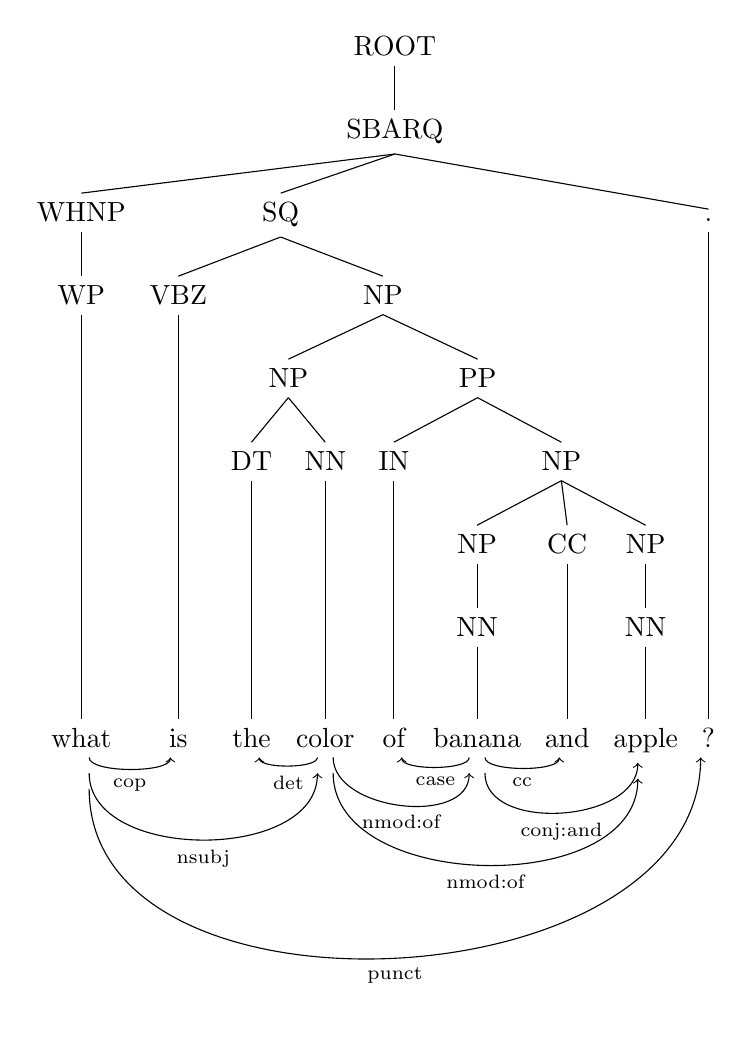
\begin{tikzpicture}
[
every edge/.style={in=270, out=270, draw=black!250}
]
\tikzset{frontier/.style={distance from root=250pt}}
\Tree [.ROOT [.SBARQ [.WHNP [.WP \node (what) {what}; ] ]
                     [.SQ [.VBZ \node (is) {is}; ]
                          [.NP [.NP [.DT \node (the) {the}; ]
                                    [.NN \node (color) {color}; ]
                               ]
                               [.PP [.IN \node (of) {of}; ]
                                    [.NP [.NP [.NN \node (banana) {banana}; ] ]
                                         [.CC \node (and) {and}; ]
                                         [.NP [.NN \node (apple) {apple}; ] ]
                                    ]
                               ]
                          ]
                     ]
                     [. . \node (qm) {?}; ]
             ]
      ]

\path[->]
([xshift=1mm, yshift=0mm] what.south)	edge[looseness=0.50] node[below] {\scriptsize cop}	([xshift=-1mm, yshift=0mm] is.south)
([xshift=-1mm, yshift=0mm] color.south)	edge[looseness=0.50] node[below] {\scriptsize det}	([xshift=1mm, yshift=0mm] the.south)
([xshift=-1mm, yshift=0mm] banana.south)	edge[looseness=0.50] node[below] {\scriptsize case}	([xshift=1mm, yshift=0mm] of.south)
([xshift=1mm, yshift=0mm] banana.south)	edge[looseness=0.50] node[below] {\scriptsize cc}	([xshift=-1mm, yshift=0mm] and.south)
([xshift=1mm, yshift=-2mm] what.south)	edge[looseness=1.00] node[below] {\scriptsize nsubj}	([xshift=-1mm, yshift=-2mm] color.south)
([xshift=1mm, yshift=0mm] color.south)	edge[looseness=1.00] node[below] {\scriptsize nmod:of}	([xshift=-1mm, yshift=-2mm] banana.south)
([xshift=1mm, yshift=-2mm] banana.south)	edge[looseness=1.00] node[below] {\scriptsize conj:and}	([xshift=-1mm, yshift=0mm] apple.south)
([xshift=1mm, yshift=-2mm] color.south)	edge[looseness=1.00] node[below] {\scriptsize nmod:of}	([xshift=-1mm, yshift=-2mm] apple.south)
([xshift=1mm, yshift=-4mm] what.south)	edge[looseness=1.03] node[below] {\scriptsize punct}	([xshift=-1mm, yshift=0mm] qm.south);
\end{tikzpicture}

      \end{adjustbox}
      \caption{Question}
    \end{subfigure}
  }
  &
  \adjustbox{valign=b}{\begin{tabular}{@{}c@{}}
    \begin{subfigure}{0.23\textwidth}\centering
      \begin{adjustbox}{scale=0.6}
        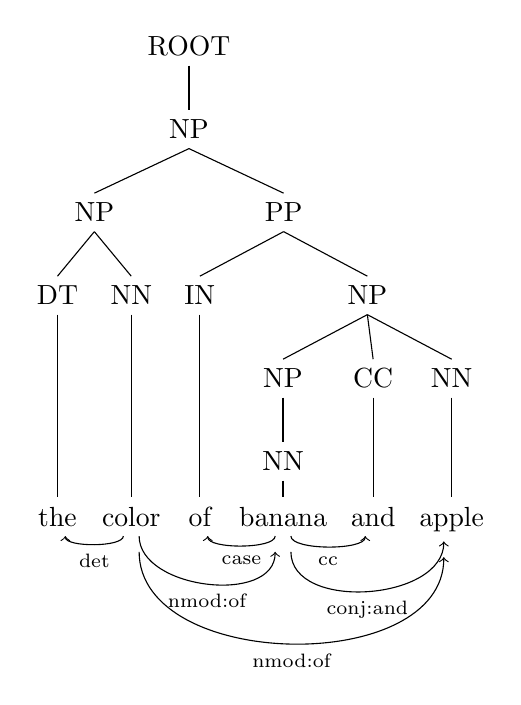
\begin{tikzpicture}
[
every edge/.style={in=270, out=270, draw=black!250}
]
\tikzset{frontier/.style={distance from root=170pt}}
\Tree [.ROOT [.NP [.NP [.DT \node (the) {the}; ]
                       [.NN \node (color) {color}; ]
                  ]
                  [.PP [.IN \node (of) {of}; ]
                       [.NP [.NP [.NN \node (banana) {banana}; ] ]
                            [.CC \node (and) {and}; ]
                            [.NN \node (apple) {apple}; ]
                       ]
                  ]
             ]
      ]

\path[->]
([xshift=-1mm, yshift=0mm] color.south)	edge[looseness=0.50] node[below] {\scriptsize det}	([xshift=1mm, yshift=0mm] the.south)
([xshift=-1mm, yshift=0mm] banana.south)	edge[looseness=0.50] node[below] {\scriptsize case}	([xshift=1mm, yshift=0mm] of.south)
([xshift=1mm, yshift=0mm] banana.south)	edge[looseness=0.50] node[below] {\scriptsize cc}	([xshift=-1mm, yshift=0mm] and.south)
([xshift=1mm, yshift=0mm] color.south)	edge[looseness=1.00] node[below] {\scriptsize nmod:of}	([xshift=-1mm, yshift=-2mm] banana.south)
([xshift=1mm, yshift=-2mm] banana.south)	edge[looseness=1.00] node[below] {\scriptsize conj:and}	([xshift=-1mm, yshift=0mm] apple.south)
([xshift=1mm, yshift=-2mm] color.south)	edge[looseness=1.00] node[below] {\scriptsize nmod:of}	([xshift=-1mm, yshift=-2mm] apple.south);
\end{tikzpicture}

      \end{adjustbox}
      \caption{Sentence}
    \end{subfigure}\\
    \begin{subfigure}{0.23\textwidth}\centering
      \begin{adjustbox}{scale=0.6}
        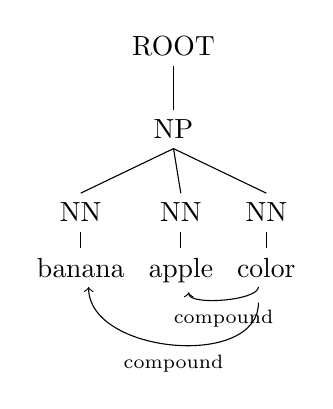
\begin{tikzpicture}
[
every edge/.style={in=270, out=270, draw=black!250}
]
\tikzset{frontier/.style={distance from root=80pt}}
\Tree [.ROOT [.NP [.NN \node (banana) {banana}; ]
                  [.NN \node (apple) {apple}; ]
                  [.NN \node (color) {color}; ]
             ]
      ]

\path[->]
([xshift=-1mm, yshift=0mm] color.south)	edge[looseness=0.50] node[below] {\scriptsize compound}	([xshift=1mm, yshift=0mm] apple.south)
([xshift=-1mm, yshift=-2mm] color.south)	edge[looseness=1.00] node[below] {\scriptsize compound}	([xshift=1mm, yshift=0mm] banana.south);
\end{tikzpicture}

      \end{adjustbox}
      \caption{Words}
    \end{subfigure}
  \end{tabular}}
  \end{tabular}
  \caption{Syntax Analysis Tree}\label{fig:dummy}
\end{figure}

% \begin{figure*}[h]
%     % \centering
%     \begin{subfigure}{0.43\textwidth}\centering
%       \begin{adjustbox}{raise=0mm,scale=0.7}
%         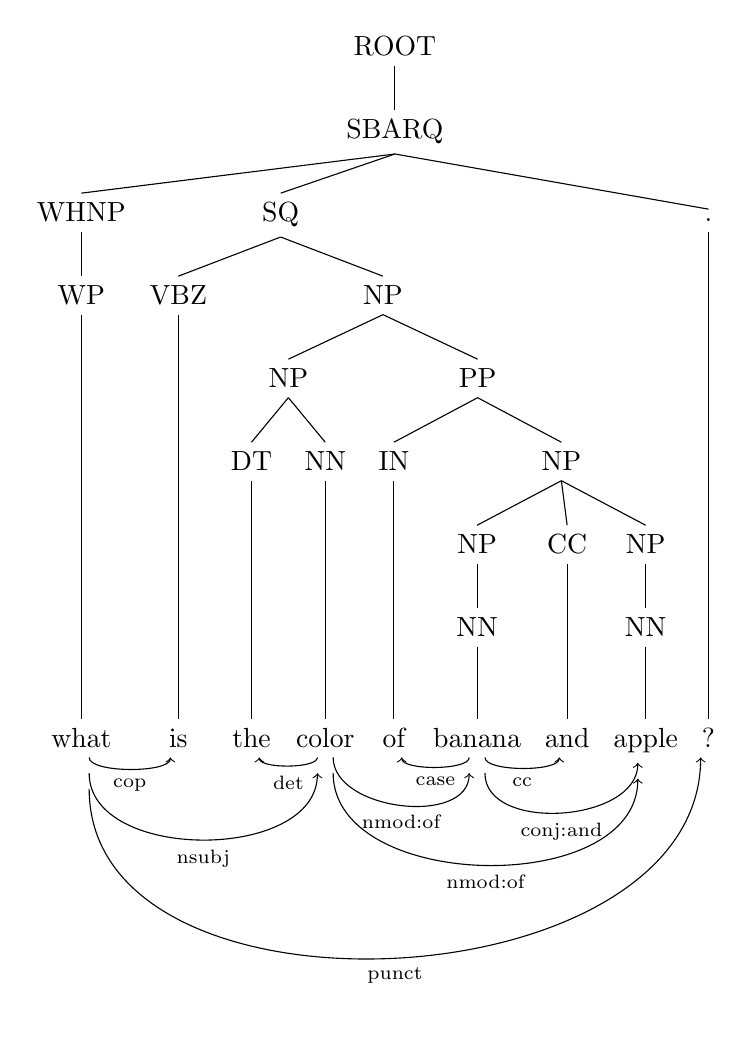
\begin{tikzpicture}
[
every edge/.style={in=270, out=270, draw=black!250}
]
\tikzset{frontier/.style={distance from root=250pt}}
\Tree [.ROOT [.SBARQ [.WHNP [.WP \node (what) {what}; ] ]
                     [.SQ [.VBZ \node (is) {is}; ]
                          [.NP [.NP [.DT \node (the) {the}; ]
                                    [.NN \node (color) {color}; ]
                               ]
                               [.PP [.IN \node (of) {of}; ]
                                    [.NP [.NP [.NN \node (banana) {banana}; ] ]
                                         [.CC \node (and) {and}; ]
                                         [.NP [.NN \node (apple) {apple}; ] ]
                                    ]
                               ]
                          ]
                     ]
                     [. . \node (qm) {?}; ]
             ]
      ]

\path[->]
([xshift=1mm, yshift=0mm] what.south)	edge[looseness=0.50] node[below] {\scriptsize cop}	([xshift=-1mm, yshift=0mm] is.south)
([xshift=-1mm, yshift=0mm] color.south)	edge[looseness=0.50] node[below] {\scriptsize det}	([xshift=1mm, yshift=0mm] the.south)
([xshift=-1mm, yshift=0mm] banana.south)	edge[looseness=0.50] node[below] {\scriptsize case}	([xshift=1mm, yshift=0mm] of.south)
([xshift=1mm, yshift=0mm] banana.south)	edge[looseness=0.50] node[below] {\scriptsize cc}	([xshift=-1mm, yshift=0mm] and.south)
([xshift=1mm, yshift=-2mm] what.south)	edge[looseness=1.00] node[below] {\scriptsize nsubj}	([xshift=-1mm, yshift=-2mm] color.south)
([xshift=1mm, yshift=0mm] color.south)	edge[looseness=1.00] node[below] {\scriptsize nmod:of}	([xshift=-1mm, yshift=-2mm] banana.south)
([xshift=1mm, yshift=-2mm] banana.south)	edge[looseness=1.00] node[below] {\scriptsize conj:and}	([xshift=-1mm, yshift=0mm] apple.south)
([xshift=1mm, yshift=-2mm] color.south)	edge[looseness=1.00] node[below] {\scriptsize nmod:of}	([xshift=-1mm, yshift=-2mm] apple.south)
([xshift=1mm, yshift=-4mm] what.south)	edge[looseness=1.03] node[below] {\scriptsize punct}	([xshift=-1mm, yshift=0mm] qm.south);
\end{tikzpicture}

%       \end{adjustbox}
%       \caption{Question}
%     \end{subfigure}
%     \hspace{-4em}
%     \begin{subfigure}{0.3\textwidth}\centering
%       \begin{adjustbox}{margin=0mm 1.50cm 0mm 1.75cm, scale=0.7}
%         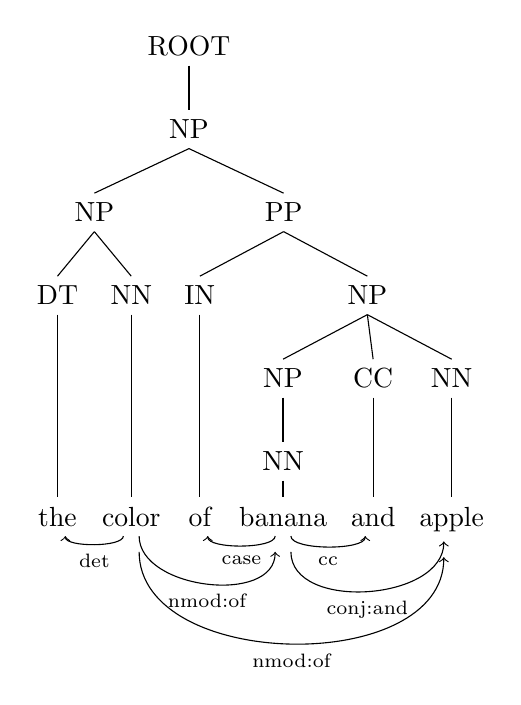
\begin{tikzpicture}
[
every edge/.style={in=270, out=270, draw=black!250}
]
\tikzset{frontier/.style={distance from root=170pt}}
\Tree [.ROOT [.NP [.NP [.DT \node (the) {the}; ]
                       [.NN \node (color) {color}; ]
                  ]
                  [.PP [.IN \node (of) {of}; ]
                       [.NP [.NP [.NN \node (banana) {banana}; ] ]
                            [.CC \node (and) {and}; ]
                            [.NN \node (apple) {apple}; ]
                       ]
                  ]
             ]
      ]

\path[->]
([xshift=-1mm, yshift=0mm] color.south)	edge[looseness=0.50] node[below] {\scriptsize det}	([xshift=1mm, yshift=0mm] the.south)
([xshift=-1mm, yshift=0mm] banana.south)	edge[looseness=0.50] node[below] {\scriptsize case}	([xshift=1mm, yshift=0mm] of.south)
([xshift=1mm, yshift=0mm] banana.south)	edge[looseness=0.50] node[below] {\scriptsize cc}	([xshift=-1mm, yshift=0mm] and.south)
([xshift=1mm, yshift=0mm] color.south)	edge[looseness=1.00] node[below] {\scriptsize nmod:of}	([xshift=-1mm, yshift=-2mm] banana.south)
([xshift=1mm, yshift=-2mm] banana.south)	edge[looseness=1.00] node[below] {\scriptsize conj:and}	([xshift=-1mm, yshift=0mm] apple.south)
([xshift=1mm, yshift=-2mm] color.south)	edge[looseness=1.00] node[below] {\scriptsize nmod:of}	([xshift=-1mm, yshift=-2mm] apple.south);
\end{tikzpicture}

%       \end{adjustbox}
%       \caption{Sentence}
%     \end{subfigure}
%     \hspace{-4em}
%     \begin{subfigure}{0.2\textwidth}\centering
%       \begin{adjustbox}{margin=0mm 2.0cm 0mm 1.75cm, scale=0.7}
%         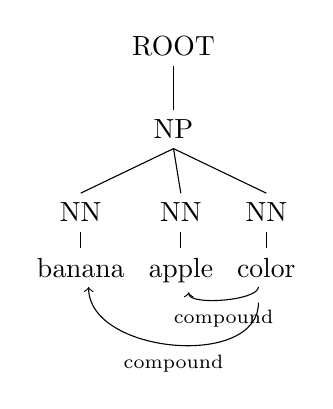
\begin{tikzpicture}
[
every edge/.style={in=270, out=270, draw=black!250}
]
\tikzset{frontier/.style={distance from root=80pt}}
\Tree [.ROOT [.NP [.NN \node (banana) {banana}; ]
                  [.NN \node (apple) {apple}; ]
                  [.NN \node (color) {color}; ]
             ]
      ]

\path[->]
([xshift=-1mm, yshift=0mm] color.south)	edge[looseness=0.50] node[below] {\scriptsize compound}	([xshift=1mm, yshift=0mm] apple.south)
([xshift=-1mm, yshift=-2mm] color.south)	edge[looseness=1.00] node[below] {\scriptsize compound}	([xshift=1mm, yshift=0mm] banana.south);
\end{tikzpicture}

%       \end{adjustbox}
%       \caption{Words}
%     \end{subfigure}
%     \caption{Syntax Analysis Tree}\label{subfig:words-query}
% \end{figure*}


As for the implementation part, we use spaCy and one of its plugins ``Berkeley Neural Parser'' to get the Constituency Parse's and Dependencies Parse's results of the sentence.


\subsection{SQuAD Dataset} \label{subsec:squad}
The Stanford Question Answering Dataset (SQuAD)\cite{rajpurkar2016squad} is designed for reading-understanding tasks. However, by utilizing this dataset, our goal is to find the important parts of given sentences and increase the corresponding weights when applying TF--IDF. In this dataset, the answer field comes from the original text, so we can take the answers in the original text as questionable and therefore, important parts. Furthermore, answer fields are represented as spans in the original text, so we can convert those spans into label sequences. Finally, we can use these two sequences (original text sequence and label sequence) to train the BiLSTM-CRF Model for sequence labeling tasks.

\begin{figure}[h]
    \centering
    \begin{lstlisting}
Born and raised in Houston, Texas, she performed in various singing and dancing competitions as a child, and rose to fame in the late 1990s as lead singer of R&B girl-group Destiny's Child.
[0, 0, 0, 0, 1, 1, 1, 0, 0, 0, 0, 0, 1, 1, 1, 0, 0, 0, 0, 0, 0, 0, 0, 0, 1, 1, 1, 1, 0, 1, 1, 0, 0, 0, 0, 0, 1, 1, 1, 0]
    \end{lstlisting}
    \caption{Caption}
    \label{fig:questionable-span}
\end{figure}

\subsection{BiLSTM-CRF Model} \label{subsec:bilstm}

\begin{figure*}[h]
  \centering
  \begin{subfigure}{\textwidth}\centering
    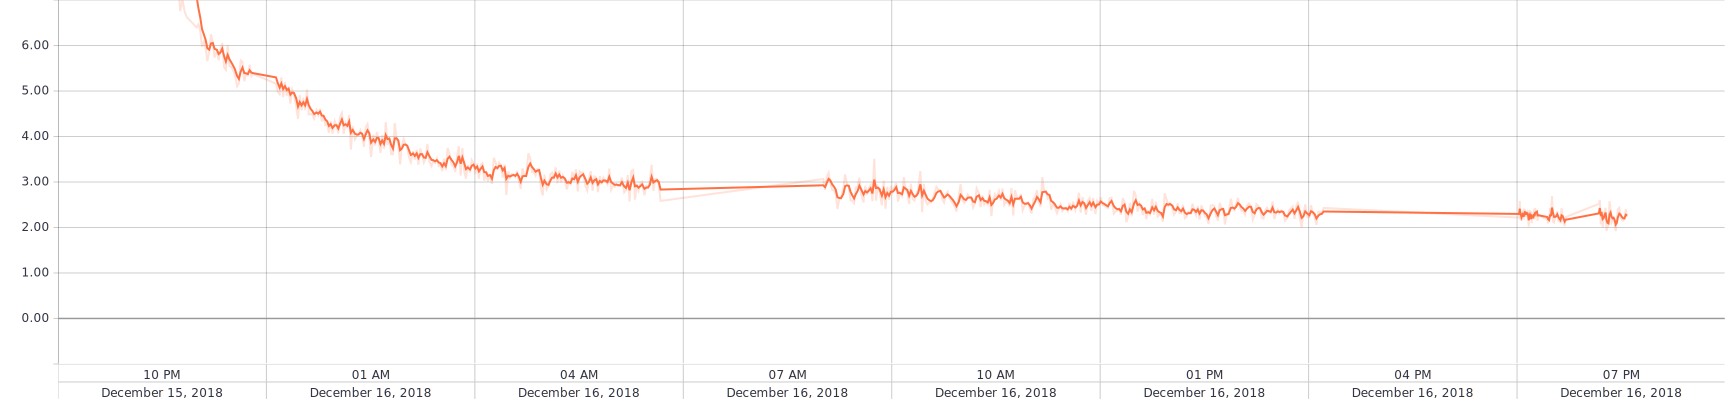
\includegraphics[width=\textwidth]{loss.pdf}
    \caption{Loss}
  \end{subfigure}\\
  \begin{subfigure}{\textwidth}\centering
    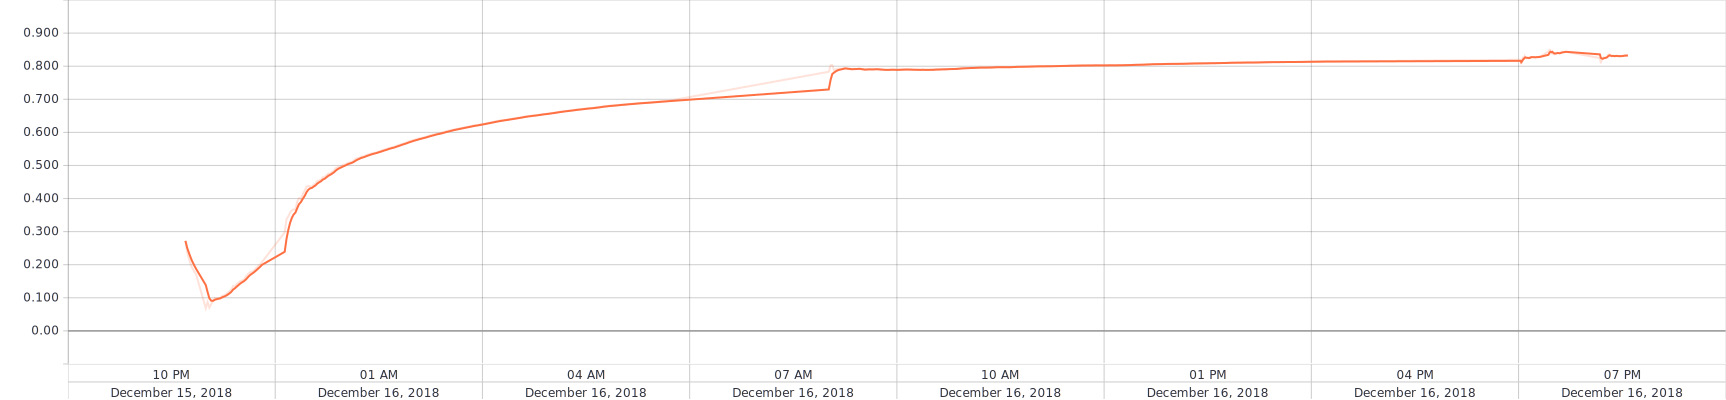
\includegraphics[width=\textwidth]{f1.pdf}
    \caption{F1}
  \end{subfigure}
  \caption{Loss and F1}
\end{figure*}

The task of finding out the ``questionable parts'' of given documents is similar to the sequence labeling task. Our task is learning a pattern to mark tokens that belong to questionable part as 1 and mark others as 0. \citeauthor{huang2015bidirectional}'s work \cite{huang2015bidirectional} inspires us to implement this part.

BiLSTM is a bidirectional version of LSTM, which generates words' representation based on the information from both forward and backward directions. LSTM is a kind of units of a recurrent neural network (RNN). A common LSTM unit is composed of a cell, an input gate, an output gate, and a forget gate. The cell remembers values over arbitrary time intervals and the three gates regulate the flow of information into and out of the cell \cite{wiki:lstm}. We use LSTM model, instead of some traditional machine learning such as random forest or AdaBoost, to make the labeling model contextualized. This is important because our task is to get a ``span'' of words instead of several scattered words as questionable parts. A contextualized model is more likely to mark a continuous sequence as 1 or 0.

The next step is to use conditional random fields (CRFs) to mark the questionable parts. CRF is a kind of sequence model used to predict labels for a sample sequence with context information. Specifically, CRF is very useful in applications such as POS Tagging, named entity recognition, etc., being an alternative to the related hidden Markov models (HMMs). Those applications are related to our task of giving 0--1 labels to tokens. It is proved that combining CRFs and BiLSTM is one of the best and most efficient ways for sequence labeling. CRF works in a similar way as Hidden Markov Model (HMM), predicting the most possible label paths of a given sequence by calculating the global conditional transfer probabilities, so that our model takes global information into consideration.

% insert model training process and result

Due to the limitation of computing resources and the amount of training data we have, this is not the final evaluation of our BiLSTM-CRF model. We look forward to better performance of this model.

\subsection{Weighted TF--IDF} \label{subsec:wtf}

TF--IDF (term frequency--inverse document frequency) is a popular term weighting scheme intended to show the importance of a word to a document in a set of documents. Given a user query, accumulating TF--IDF values of each term in the query gets different scores for different documents, which shows the relevance between the query and the documents.

TF--IDF is the product of TF (term frequency) and IDF (inverse document frequency). TF simply shows the number of times a term occurs in a document, while IDF helps to diminishes the weight of discriminative terms like ``the'' hence to increase the weight of terms that occur rarely in the whole corpus. TF and IDF can be calculated as
\begin{align*}
    \text{tf} (t,d) &= \text{count} (t,d) \,, \\
    \mathrm{idf}(t, D) &= \log \frac{|D|}{1+|\{d \in D: t \in d\}|} \,,
\end{align*}
where $\text{count} (t,d)$ is the number of times term $t$ occurs in document $d$, $|D|$ is the total number of documents in the corpus $D$, and
$|\{d \in D: t \in d\}|$ is the number of documents where the term $t$ appears. Thus, TF--IDF can be calculated as
\begin{displaymath}
    \text{tfidf} (t,d,D)=\text{tf} (t,d)\cdot \text{idf} (t,D) \,.
\end{displaymath}

Although IDF catches the importance of a term in a corpus and diminishes influences from discriminative terms, it determines the amount of information a word contains based on a corpus-wide evaluation. With the intention to let our model pay even more attention to the document-wise more meaningful parts, i.e., questionable spans, we introduce Weighted TF--IDF.

Weighted TF--IDF adds a weight $w$ to TF--IDFs of terms that are included in the questionable spans of a document, so that the terms containing more meaningful information in a document contribute more to its score. We define Weighted TF--IDF as
\begin{displaymath}
    \text{w-tfidf} (t,d,D) =
    \begin{cases}
        \text{tfidf} (t,d,D) \,, & \text{if $t \notin \text{qs}_d$}\,, \\
        w \cdot \text{tfidf} (t,d,D) \,, & \text{if $t \in \text{qs}_d$}\,,
    \end{cases}
\end{displaymath}
where $\text{qs}_d$ is the questionable spans of document $d$.

Implementing the TF--IDF model, we create inverted index mapping terms in the corpus to the documents containing them in order to make a speedy search. We also create another inverted index mapping terms to the documents containing them as a token in the questionable spans, so that we can check if a TF--IDF needs to get $w$ times weighted more efficiently.

\subsection{BERT Model} \label{subsec:bert}

BERT (Bidirectional Encoder Representation from Transformers) is a state-of-the-art pre-training language representations with which we can generate the sentence embedding (like word embedding). Like ELMo\cite{Peters:2018}, BERT also uses multilayer network to capture the text meaning. However, BERT introduces self-attention mechanism and Transformer\cite{Vaswani2017AttentionIA} to encode input token, making it the best language representations model nowadays.

We use the last layer of BERT hidden layer and sum up each token's output vector into one vector used to represent sentence embedding. Notably, the token's output vectors here do not include the CLS token and the SEP token. The reason is that these two tokens play similar rols and create similar vectors even in different token sequences, which could decrease the distinction of different sentences and make it difficult for ranking.

\begin{figure*}[ht]
\centering
\tikzstyle{title} = [text width=7em]
\tikzstyle{input} = [rectangle, draw,
    text width=2em, text centered, rounded corners, node distance=1cm, minimum height=1.6em]
\tikzstyle{embed} = [rectangle, draw,
    text width=2em, text centered, node distance=1cm, minimum height=1.6em]
\tikzstyle{plus} = [text width=2em, text centered, node distance=1cm]
% \tikzstyle{line} = [draw, -latex']
% \tikzstyle{cloud} = [draw, ellipse, node distance=3cm,
%     text width=5em, text centered, minimum height=2em]

\begin{tikzpicture}[font=\footnotesize]
\node [title] (i-1) {Input};
\node [input, right of=i-1, node distance=5.5em] (i0) {[CLS]};
\node [input, right of=i0] (i1) {my};
\node [input, right of=i1] (i2) {dog};
\node [input, right of=i2] (i3) {is};
\node [input, right of=i3] (i4) {cute};
\node [input, right of=i4] (i5) {[SEP]};
\node [input, right of=i5] (i6) {he};
\node [input, right of=i6] (i7) {likes};
\node [input, right of=i7] (i8) {playing};
\node [input, right of=i8] (i9) {\#\#ING};
\node [input, right of=i9] (i10) {[SEP]};

\node [title, below of=i-1] (te-1) {Token Embeddings};
\node [embed, right of=te-1, node distance=5.5em] (te0) {$\text{E}_{\text{[CLS]}}$};
\node [embed, right of=te0] (te1) {$\text{E}_{\text{my}}$};
\node [embed, right of=te1] (te2) {$\text{E}_{\text{dog}}$};
\node [embed, right of=te2] (te3) {$\text{E}_{\text{is}}$};
\node [embed, right of=te3] (te4) {$\text{E}_{\text{cute}}$};
\node [embed, right of=te4] (te5) {$\text{E}_{\text{[SEP]}}$};
\node [embed, right of=te5] (te6) {$\text{E}_{\text{he}}$};
\node [embed, right of=te6] (te7) {$\text{E}_{\text{likes}}$};
\node [embed, right of=te7] (te8) {$\text{E}_{\text{playing}}$};
\node [embed, right of=te8] (te9) {$\text{E}_{\text{\#\#ING}}$};
\node [embed, right of=te9] (te10) {$\text{E}_{\text{[SEP]}}$};

\node [title, below of=te-1] (se-1) {Segment Embeddings};
\node [embed, right of=se-1, node distance=5.5em] (se0) {$\text{E}_{\text{A}}$};
\node [embed, right of=se0] (se1) {$\text{E}_{\text{A}}$};
\node [embed, right of=se1] (se2) {$\text{E}_{\text{A}}$};
\node [embed, right of=se2] (se3) {$\text{E}_{\text{A}}$};
\node [embed, right of=se3] (se4) {$\text{E}_{\text{A}}$};
\node [embed, right of=se4] (se5) {$\text{E}_{\text{A}}$};
\node [embed, right of=se5] (se6) {$\text{E}_{\text{B}}$};
\node [embed, right of=se6] (se7) {$\text{E}_{\text{B}}$};
\node [embed, right of=se7] (se8) {$\text{E}_{\text{B}}$};
\node [embed, right of=se8] (se9) {$\text{E}_{\text{B}}$};
\node [embed, right of=se9] (se10) {$\text{E}_{\text{B}}$};

\node [title, below of=se-1] (pe-1) {Position Embeddings};
\node [embed, right of=pe-1, node distance=5.5em] (pe0) {$\text{E}_{\text{0}}$};
\node [embed, right of=pe0] (pe1) {$\text{E}_{\text{1}}$};
\node [embed, right of=pe1] (pe2) {$\text{E}_{\text{2}}$};
\node [embed, right of=pe2] (pe3) {$\text{E}_{\text{3}}$};
\node [embed, right of=pe3] (pe4) {$\text{E}_{\text{4}}$};
\node [embed, right of=pe4] (pe5) {$\text{E}_{\text{5}}$};
\node [embed, right of=pe5] (pe6) {$\text{E}_{\text{6}}$};
\node [embed, right of=pe6] (pe7) {$\text{E}_{\text{7}}$};
\node [embed, right of=pe7] (pe8) {$\text{E}_{\text{8}}$};
\node [embed, right of=pe8] (pe9) {$\text{E}_{\text{9}}$};
\node [embed, right of=pe9] (pe10) {$\text{E}_{\text{10}}$};

\node [title, below of=te-1, node distance=1.6em] (pA-1) {};
\node [plus, right of=pA-1, node distance=5.5em] (pA0) {+};
\node [plus, right of=pA0] (pA1) {+};
\node [plus, right of=pA1] (pA2) {+};
\node [plus, right of=pA2] (pA3) {+};
\node [plus, right of=pA3] (pA4) {+};
\node [plus, right of=pA4] (pA5) {+};
\node [plus, right of=pA5] (pA6) {+};
\node [plus, right of=pA6] (pA7) {+};
\node [plus, right of=pA7] (pA8) {+};
\node [plus, right of=pA8] (pA9) {+};
\node [plus, right of=pA9] (pA10) {+};

\node [title, below of=se-1, node distance=1.6em] (pB-1) {};
\node [plus, right of=pB-1, node distance=5.5em] (pB0) {+};
\node [plus, right of=pB0] (pB1) {+};
\node [plus, right of=pB1] (pB2) {+};
\node [plus, right of=pB2] (pB3) {+};
\node [plus, right of=pB3] (pB4) {+};
\node [plus, right of=pB4] (pB5) {+};
\node [plus, right of=pB5] (pB6) {+};
\node [plus, right of=pB6] (pB7) {+};
\node [plus, right of=pB7] (pB8) {+};
\node [plus, right of=pB8] (pB9) {+};
\node [plus, right of=pB9] (pB10) {+};

\end{tikzpicture}

\caption{Bert Tokens}\label{fig:bert-token}
\end{figure*}

With the sentence embedding created by BERT, we are able to calculate the similarity of different sentence via creating sentence embedding. We call this kind of similarity as ``semantic score'', which could be used to introduce semantic information in our retrieval rank task. Because we already are able to get the weight TF--IDF score as the previous section described, the specific approach is to add this two scores together and make a final sort. It is reasonable because the information those two scores represented is orthogonal. The TF--IDF score represents the scenario that the user input exactly match the documents; the semantic score represents the scenario that user want to search some relevant documents. Even BERT is the current best model for language representations, it still is a black box model and very sensitive to noise. Moreover, a more common scenario is that user expect search result exactly matches user's input, and semantic information only is a supplement for traditional keywords searching approach. On the other hand, TF--IDF model does not take semantic information into consideration at all. It is a compromise approach to combining the two score together. If users' input is a meaningless token sequence, we should only consider the Weighted TF--IDF score.

In order to reduce the computation on similarities for all sentence pairs, we first use Weighted TF--IDF to rank documents and get a larger number of top documents than needed, say 100, as potential results. Then we use BERT to calculate the similarities between user's query and these 100 candidates, re-rank the documents and get the top 10. This helps to get results more accurately and efficiently when the corpus is very large and there are many of them getting similar TF--IDF scores. For example, if a user search with a query ``red apple'' from a corpus where there are two documents, ``the red apple is placed in the house'' and ``the apple is placed inside the red house'', TF--IDF gives the same score regardless of different semantic information. Here is where BERT comes in. With BERT, our goal is to disambiguate the top-ranked TF--IDF results and make give them a better ranking.


\section{Experiment}\label{sec:experiment}

\subsection{Setup}
To illustrate the effectiveness of our approach in improving the precision of semantic search, we would like to set up an experiment. We used the Yahoo! Answers Manner Questions v2.0 dataset as our experimental dataset, which is a subset of the Yahoo! Answers corpus from a Oct 25, 2007 dump. It is a small subset of the questions, selected for their linguistic properties. Additionally, questions and answers of obviously low quality are removed from the dataset, i.e. only questions and answers that have at least four words, out of which at least one is a noun and at least one is a verb, are kept.

We followed two steps to generate a preprocessed database. First, we used the BiLSTM-CRF model trained with the SQuAD dataset to identify all the questionable spans in the answer set of our experimental dataset. This is for the purpose of calculating the Weighted TF--IDF score later. Second, we used the BERT natural language model to convert all the sentences in the answer set into high-dimensional vectors based on their semantic distance.

We then randomly selected 1000 questions from the question set of the experiment dataset as user input queries. We used three models to compute the top 5 most relevant ranked sentences individually. These three models were the traditional TF--IDF method, the Weighted TF--IDF method and our proposed approach, the Weighted TF--IDF method combined with the BERT model.

We hid the source models of the output and let human readers to mark the relevance of the output based on the corresponding input question. With these labeled relevances, we finally used three metrics to compare the experiment results --- P@3 (Precision at 3), P@5 (Precision at 5) and NDCG (Normalized Discounted Cumulative Gain). Precision at a particular rank position $k$ is defined as
\begin{align*}
    \mbox{P@$k$} &= \frac{|\{\mbox{relevant docs}\}\cap\{\mbox{retrieved docs}\}|}{|\{\mbox{retrieved docs}\}|}  \,,
\end{align*}
and NDCG at position $p$ is defined as
\begin{displaymath}
  \text{NDCG}_p = \frac{\text{DCG}_p}{\text{IDCG}_p} \,,
\end{displaymath}
where $\text{DCG}_p=\sum_{i=1}^{p}\frac{rel_i}{\log_2(i+1)}$\,, and $\text{IDCG}_p=\sum_{i=1}^{\text{|REL|}}\frac{rel_i}{\log_2(i+1)}$\,.

\subsection{Result}

\begin{table}[h]
  \caption{Experiment Result}
  \label{tab:experiment-result}
  \begin{tabular}{lccc}
    \toprule
    \, & P@3 & P@5 & $\text{NDCG}_5$ \\
    \midrule
    TF--IDF & 0.243 & 0.214 & 0.366 \\
    Weighted TF--IDF & 0.293 & 0.272 & 0.412 \\
    Weighted TF--IDF + BERT & 0.529 & 0.501 & 0.519 \\
  \bottomrule
\end{tabular}
\end{table}

\begin{figure*}[t]
\lstinputlisting{search-eg.txt}
\caption{An example of outputs}\label{fig:example}
\end{figure*}

We provide the experiment results of the three metrics mentioned above in Table \ref{tab:experiment-result}. The numbers are the mean value computed based on the outputs of 1000 input queries using the corresponding experiment setup.

Figure \ref{fig:example} is an example of the outputs given by two different models with the same input query. The first 5 sentences are generated by our approach (Weighted TF--IDF + BERT). The other 5 sentences are generated by the traditional TF--IDF method.

\subsection{Evaluation}
As reflected in the Table \ref{tab:experiment-result}, our proposed Weighted TF--IDF method outperforms the traditional TF--IDF method in all three metrics. This shows that by identifying the questionable spans in the text and give them higher weights when calculating the TF--IDF score, we are more capable of finding the most relevant answers to user queries.

Moreover, the BERT natural language model aids the Weighted TF--IDF method in terms of providing semantic relevance measures so as to better compare the true semantics between the user query and potential answers. As we can see in Table \ref{tab:experiment-result}, the model of the Weighted TF--IDF method together with the BERT model outperforms the traditional TF--IDF method by a significant margin in all three metrics.

We provide a sample output generated by these two models in Figure \ref{fig:example}. There are 3 sentences in the results of our proposed model that are considered semantically relevant to the user query. In contrast, there is only 1 sentence in the results of the traditional TF--IDF method that is perceived as semantically relevant to the user input. This well illustrates that our proposed model indeed improves the semantic search precision as compared to the traditional TF--IDF method.

However, the precision and cumulative gain we get from both our proposed approach and the traditional TF--IDF method are still quite low. We believe that it is caused by the diverse nature and relatively small size of the experiment dataset. There may not be enough semantically similar documents in the dataset, which means that even a perfect semantic search engine cannot find 5 relevant answers to all the user input queries. Nonetheless, our proposed approach still outperforms existing methods by a significant margin and is able to rank the results properly according to their relevance.

\section{Conclusion} \label{sec:conclusion}
In this paper, we defined a new concept of ``Questionable Spans'' which refers to the parts in a text that stands a high chance of forming the answer to a question targeting the original text. Given that, we proposed a novel approach which identifies the questionable spans in a sentence and gives higher weights to them when calculating the TF--IDF score. We then incorporate the BERT natural language model to complement the TF--IDF framework in terms of providing true semantic relevance measures of potential answers during a semantic search. Based on our experiment results, our proposed approach outperforms existing methods like the traditional TF--IDF method by a significant margin in both the precision and cumulative gain of the search results.

We plan to extend our proposed approach in several ways in the future: bringing in more features such as the depth of the word in the syntax tree when training the BiLSTM-CRF model, and extending the BERT model to handle the case when users input a sequence of words instead of a complete sentence.

% \input{samplebody-conf.tex}

% \bibliographystyle{ACM-Reference-Format}
% \bibliography{bibliography.bib}


\end{document}
